\chapter{Исследовательская часть}

\section{Технические характеристики}
Характеристики используемого оборудования:
\begin{itemize}
    \item[---] Операционная система --- Windows 11 Home [6]
    \item[---] Память --- 16 Гб.
    \item[---] Процессор --- Intel(R) Core(TM) i5-10300H CPU @ 2.50Ггц [7]
    \item[---] Микроконтроллер --- STM32F303 [8]
\end{itemize}

\section{Описание используемых типов данных}
Используемые типы данных:

размер матрицы --- целое число типа $size\_t$;

матрица --- $std::vector$< $std::vector$<$int$> >.


\clearpage

\section{Время выполнения алгоритмов}
Результаты замеров времени работы трех алгоритмов умножения матриц приведены в таблице \ref{tbl:time_measurements}. Время работы замерялось на микроконтроллере STM32F303 с тактовой частотой до 72 Мгц. Замеры времени проводились на матрицах одинаковой длины и усреднялись для каждого набора одинаковых экспериментов. Каждое значение получено путем взятия среднего из 100 измерений. Зависимости времени умножения от размера матрицы для трех алгоритмов представлены на рисунке \ref{fig:tm}.

\begin{table}[h]
	\begin{center}
		\begin{threeparttable}
		\captionsetup{justification=raggedright,singlelinecheck=off}
		\caption{Время работы алгоритмов (в мс)}
		\label{tbl:time_measurements}
		\begin{tabular}{|c|c|c|c|c|}
			\hline
			Размер матрицы &  Классический & Виноград & Виноград (оптимизированный) \\
            \hline
			1    & 0.12 & 0.34 & 0.30 \\
            \hline
			2    & 0.55 & 0.52 & 0.50 \\ 
            \hline
			4    & 1.05 & 0.62 & 0.52 \\ 
            \hline
			8    & 1.56 & 1.56 & 1.50 \\ 
			\hline
			10    & 4.68 & 3.36 & 2.08 \\ 
			\hline
			20    & 28.60 & 4.16 & 19.76 \\ 
			\hline
			21    & 96.72 & 25.48 & 21.84 \\ 
			\hline
			32    & 299.00 & 92.04 & 76.96 \\ 
			\hline
			43    & 498.16 & 197.08 & 172.64 \\ 
			\hline
			54    & 890.24 & 417.56 & 359.32 \\ 
			\hline
			65    & 1628.64 & 777.40 & 670.28 \\ 
			\hline
            76    & 2272.40 & 1161.16 & 991.12 \\ 
            \hline
            87    & 3104.16 & 1944.80 & 1682.20 \\ 
            \hline
            98   & 3307.20 & 2643.16 & 2276.04 \\ 
            \hline
		\end{tabular}
		\end{threeparttable}
    \end{center}
\end{table}

\begin{figure}[H]
    \centering
    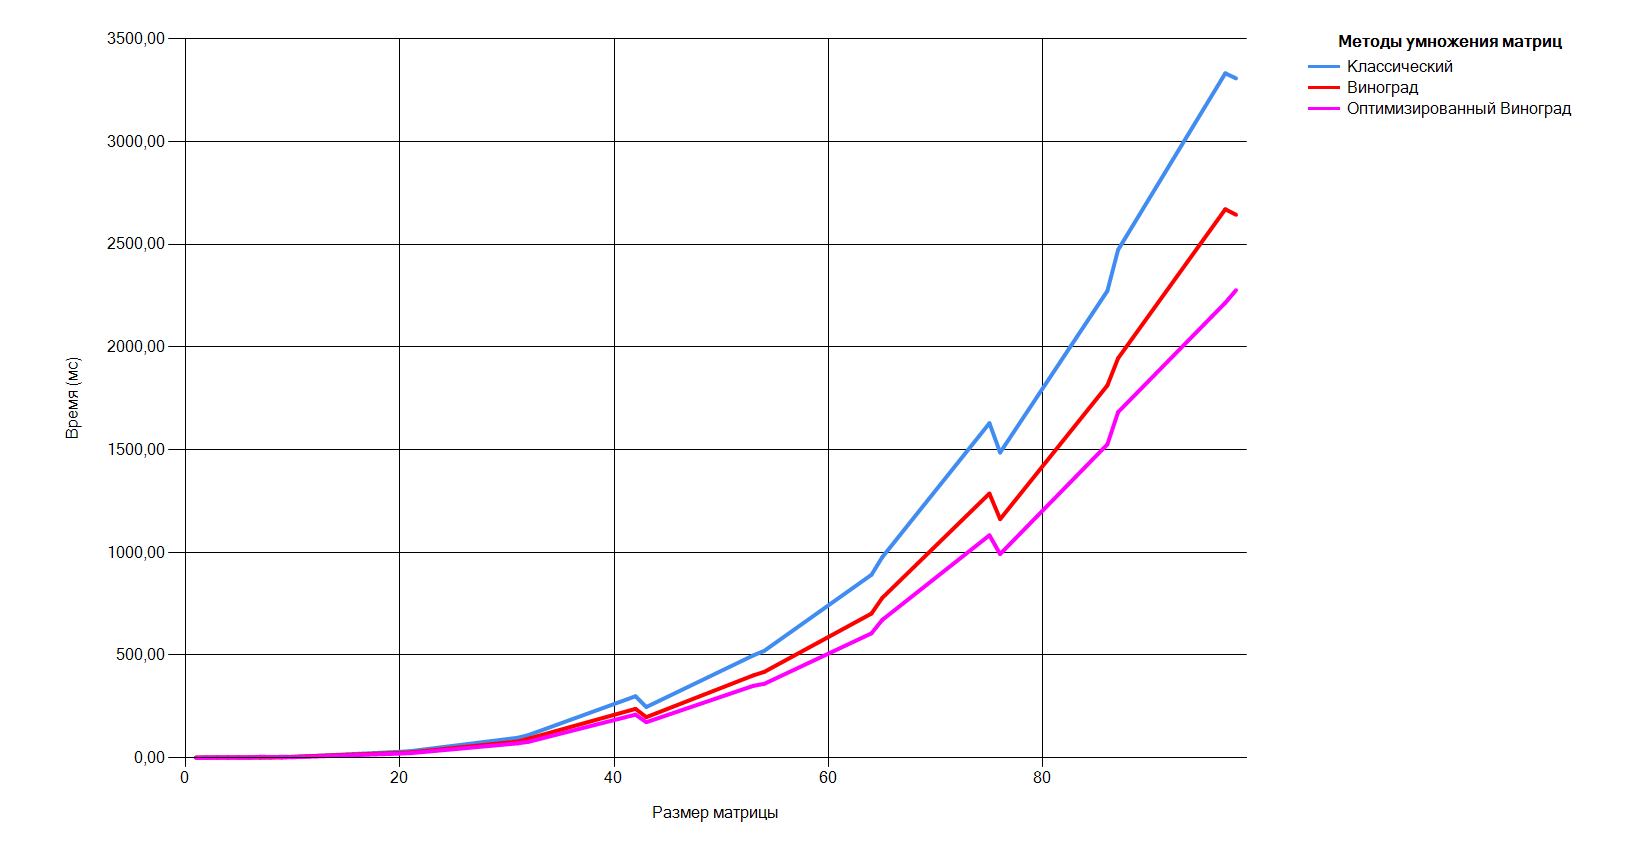
\includegraphics[width=1\linewidth]{img/graph.png}
    \caption{Сравнение алгоритмов по времени}
    \label{fig:tm}
\end{figure}

\clearpage

\section{Вывод}

В результате исследования было получено, что при больших размерах матриц (свыше 10), алгоритм Винограда работает быстрее стандартного алгоритма более, чем 1.2 раза, а оптимизированный алгоритм Винограда быстрее стандартного алгоритма почти в 1.5 раза. В итоге, можно сказать, что при таких данных следует использовать оптимизированный алгоритм Винограда.

Также было выявлено, что на четных размерах реализация алгоритма Винограда работает быстрее, чем на нечетных размерах матриц, что обусловлено необходимостью проводить дополнительные вычисления для крайних строк и столбцов. Следовательно, стоит использовать алгоритм Винограда для матриц, которые имеют четные размеры.